% Graphic: Análise de tempo nos resultados do Experimento Delta
% \begin{figure*}[!ht]
\begin{figure}[H]
\centering
	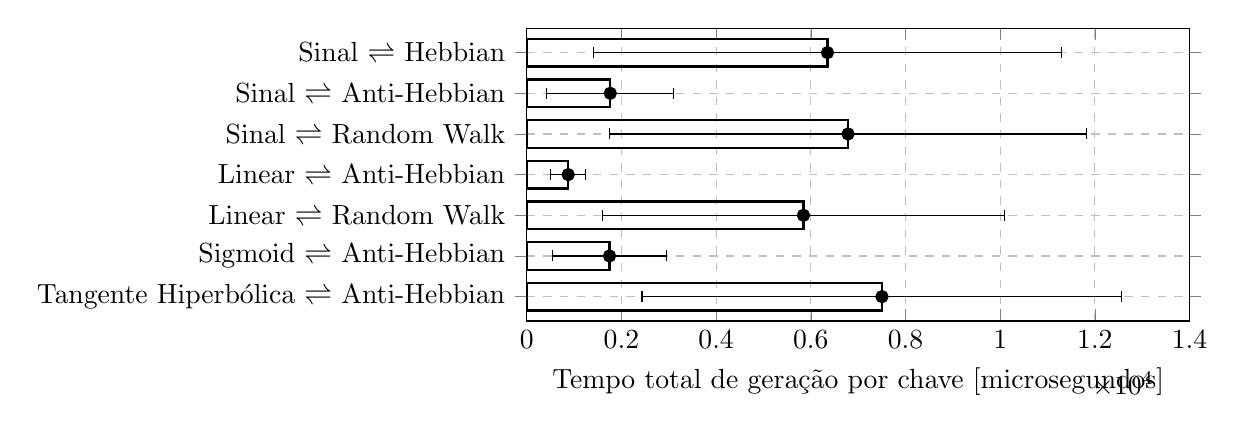
\begin{tikzpicture}
		\begin{axis}[
			%title={Número médio de épocas de treinamento com desvio padrão no Experimento $\delta$},
			tick scale binop=\times,
			symbolic y coords={Tangente Hiperbólica $\rightleftharpoons$ Anti-Hebbian, Sigmoid $\rightleftharpoons$ Anti-Hebbian, Linear $\rightleftharpoons$ Random Walk, Linear $\rightleftharpoons$ Anti-Hebbian, Sinal $\rightleftharpoons$ Random Walk, Sinal $\rightleftharpoons$ Anti-Hebbian, Sinal $\rightleftharpoons$ Hebbian},
			xbar,
			xmin=0,
			xlabel={Tempo total de geração por chave [microsegundos]},
			bar width=10pt,
			ytick=data,
			legend pos=north east,
			ymajorgrids=true,
			xmajorgrids=true,
			grid style=dashed,
			height=5.3cm,
			width=10cm,
			xmin=0, xmax=14000,
			%nodes near coords, nodes near coords align={horizontal},
		]
		 
		\addplot[color=black, solid, thick, mark=*] plot[error bars/.cd, x dir=both, x explicit]
			coordinates {
				(6352,Sinal $\rightleftharpoons$ Hebbian) +- (4947.3,7756.7)
				(1765,Sinal $\rightleftharpoons$ Anti-Hebbian) +- (1341.1,2188.9)
				(6787,Sinal $\rightleftharpoons$ Random Walk) +- (5041.8,8532.2)
				(876,Linear $\rightleftharpoons$ Anti-Hebbian) +- (374.4,1377.6)
				(5845,Linear $\rightleftharpoons$ Random Walk) +- (4244.4,7445.6)
				(1748,Sigmoid $\rightleftharpoons$ Anti-Hebbian) +- (1196.1,2299.9)
				(7503,Tangente Hiperbólica $\rightleftharpoons$ Anti-Hebbian) +- (5068.3,9937.7)
			}; %\legend{Tempo em microsegundos}
		 
		\end{axis}
	\end{tikzpicture}
	\caption{Análise do tempo médio total de geração por chave com desvio padrão nos resultados do Experimento 1.}
	\label{graph:timeResultsDelta}
\end{figure}